\documentclass[12pt,titlepage]{article}
\usepackage[margin=1.25in]{geometry}
\usepackage{graphicx,amsmath,blindtext,minted}
% Variables definition
\newcommand{\vSubject}{Advanced Web Programming}
\newcommand{\vSubtitle}{RESTFUL API}
\newcommand{\vName}{Muhammad Baihaqi Aulia Asy'ari}
\newcommand{\vNIM}{2241720145}
\newcommand{\vClass}{2I}
\newcommand{\vDepartment}{Information Technology}
\newcommand{\vStudyProgram}{D4 Informatics Engineering}
% [START] Tikz related stuff
\usepackage{tikz}
\usetikzlibrary{svg.path,calc,shapes.geometric,shapes.misc}
\tikzstyle{terminator} = [rectangle, draw, text centered, rounded corners = 1em, minimum height=2em]
\tikzstyle{preparation} = [chamfered rectangle, chamfered rectangle sep=0.75em, draw, text centered, minimum height = 2em]
\tikzstyle{process} = [rectangle, draw, text centered, minimum height=2em]
\tikzstyle{decision} = [diamond, aspect=2, draw, text centered, minimum height=2em]
\tikzstyle{data}=[trapezium, draw, text centered, trapezium left angle=60, trapezium right angle=120, minimum height=2em]
% [END] Tikz related stuff
% [START] Fancy header related stuff
\usepackage{fancyhdr}
\pagestyle{fancy}
\setlength{\headheight}{15pt}
\fancyhead{}
\fancyfoot{}
\fancyfoot[L]{\thepage}
\fancyfoot[R]{\textit{\vSubject - \vSubtitle}}
\renewcommand{\footrulewidth}{0.4pt}
% [END] Fancy header related stuff
% [START] Custom tabular command related stuff
\usepackage{tabularx}
\newcommand{\details}[2]{
    #1 
}
% [END] Custom tabular command related stuff
% [START] Figure related stuff
\newcommand{\image}[3][1]{
    \begin{figure}[h]
        \centering
        \includegraphics[#1]{#2}
        \caption{#3}
        \label{#3}
    \end{figure}
}
% [END] Figure related stuff
%
\usepackage{pgf-umlcd}
\renewcommand{\umldrawcolor}{black}
\renewcommand{\umlfillcolor}{white}
%
% [BEGIN] Custom enumerator
\usepackage{enumitem}
% [END] Custom enumerator
% [BEGIN] Paragraph indent
\usepackage{indentfirst}
% [END] Paragraph indent
% [BEGIN] URL
\usepackage{hyperref}
\hypersetup{
    colorlinks=true,
    linkcolor=blue,
    filecolor=magenta,      
    urlcolor=cyan,
    pdftitle={Overleaf Example},
    pdfpagemode=FullScreen,
    }
\urlstyle{same}
% [END] URL
\begin{document}
\begin{titlepage}
    \centering
    \vfill
    {\bfseries\LARGE
        \vSubject\\
        \vskip0.25cm
        \vSubtitle
    }
    \vfill
    
\includegraphics[width=6cm]{images/polinema-logo.png}
    \vfill
    {
        \textbf{Name}\\
        \vName\\
        \vskip0.5cm
        \textbf{NIM}\\
        \vNIM\\
        \vskip0.5cm
        \textbf{Class}\\
        \vClass\\
        \vskip0.5cm
        \textbf{Department}\\
        \vDepartment\\
        \vskip0.5cm
        \textbf{Study Program}\\
        \vStudyProgram
    }
\end{titlepage}
\newpage
\section{Practicum 1 - Creating a RESTful API Register}
\begin{enumerate}
    \item[11.] - \\ 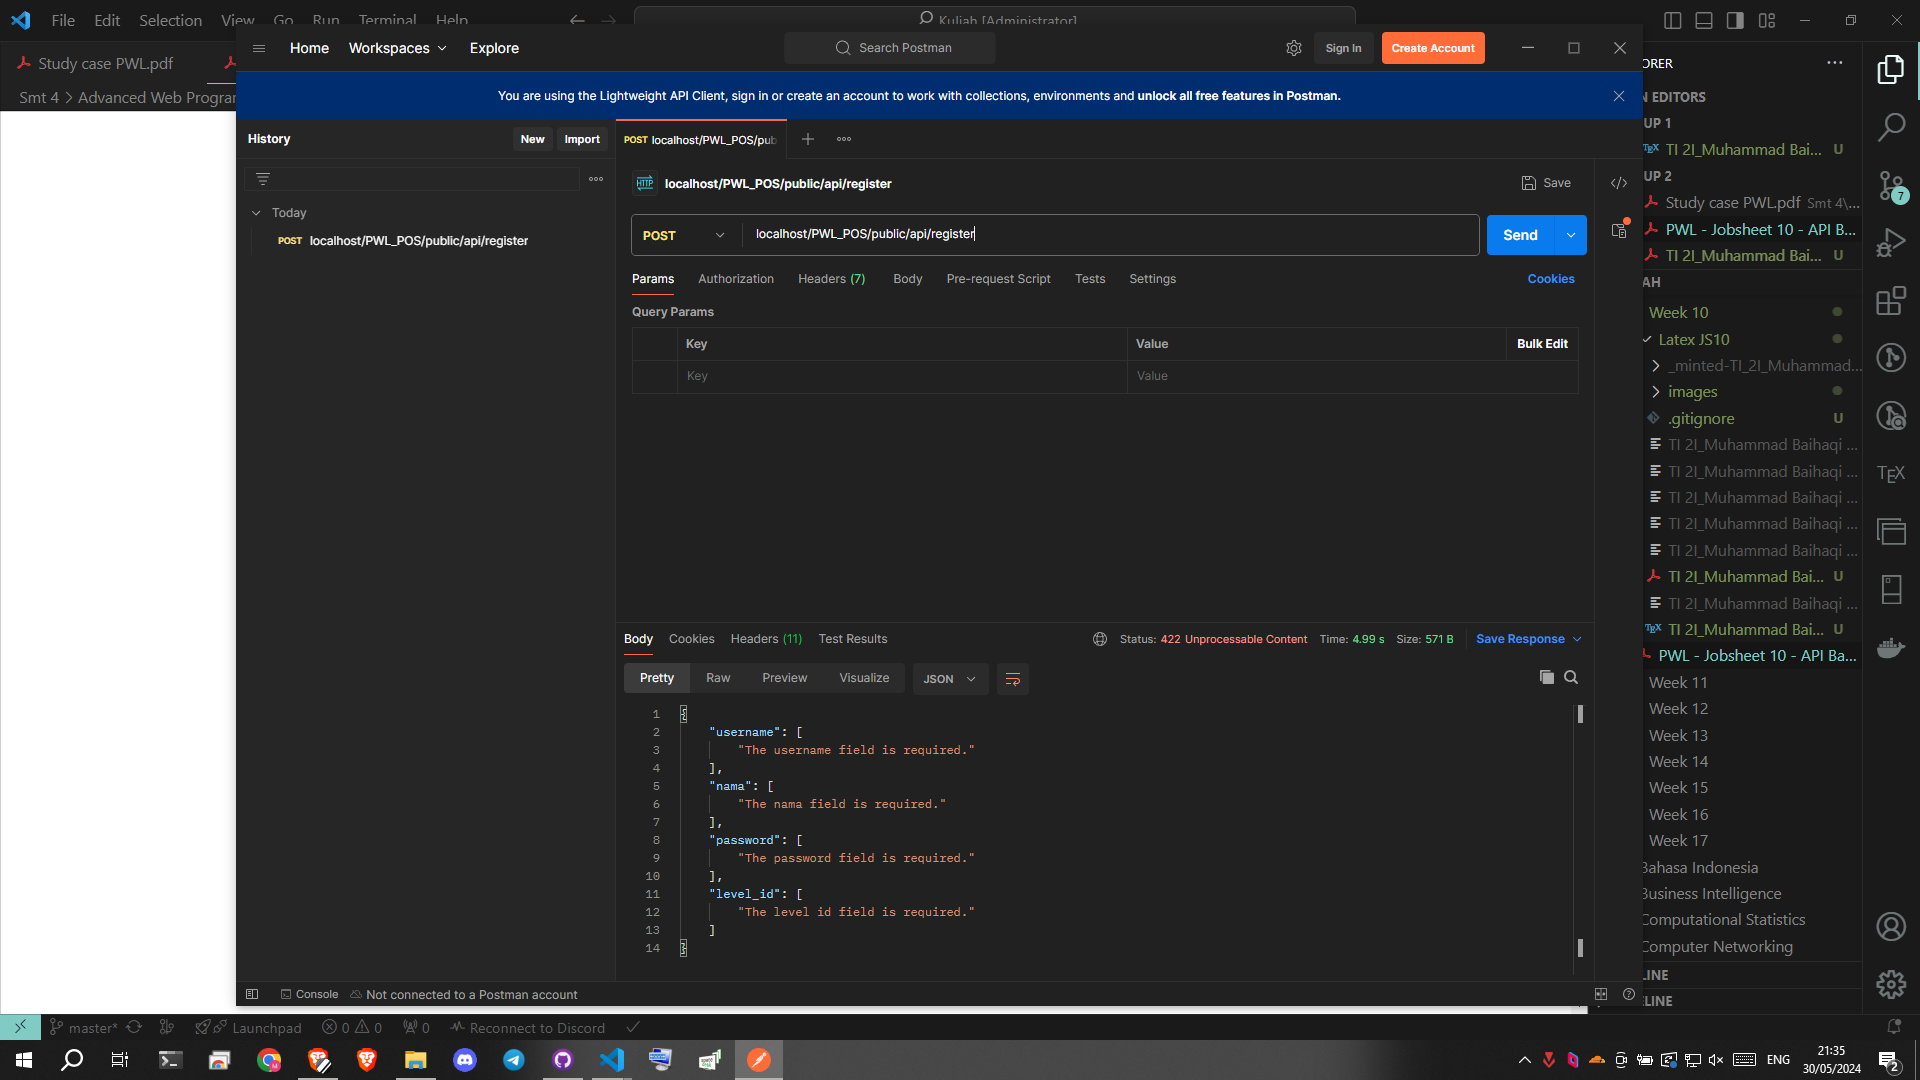
\includegraphics[width=.9\textwidth]{images/figures/Screenshot (474).png}
\end{enumerate}
\section{Practicum 2 - Creating a RESTful API Login}
\begin{enumerate}
    \item[4.] - \\ \includegraphics[width=.9\textwidth]{images/figures/Screenshot (475).png}
    \item[5.] - \\ 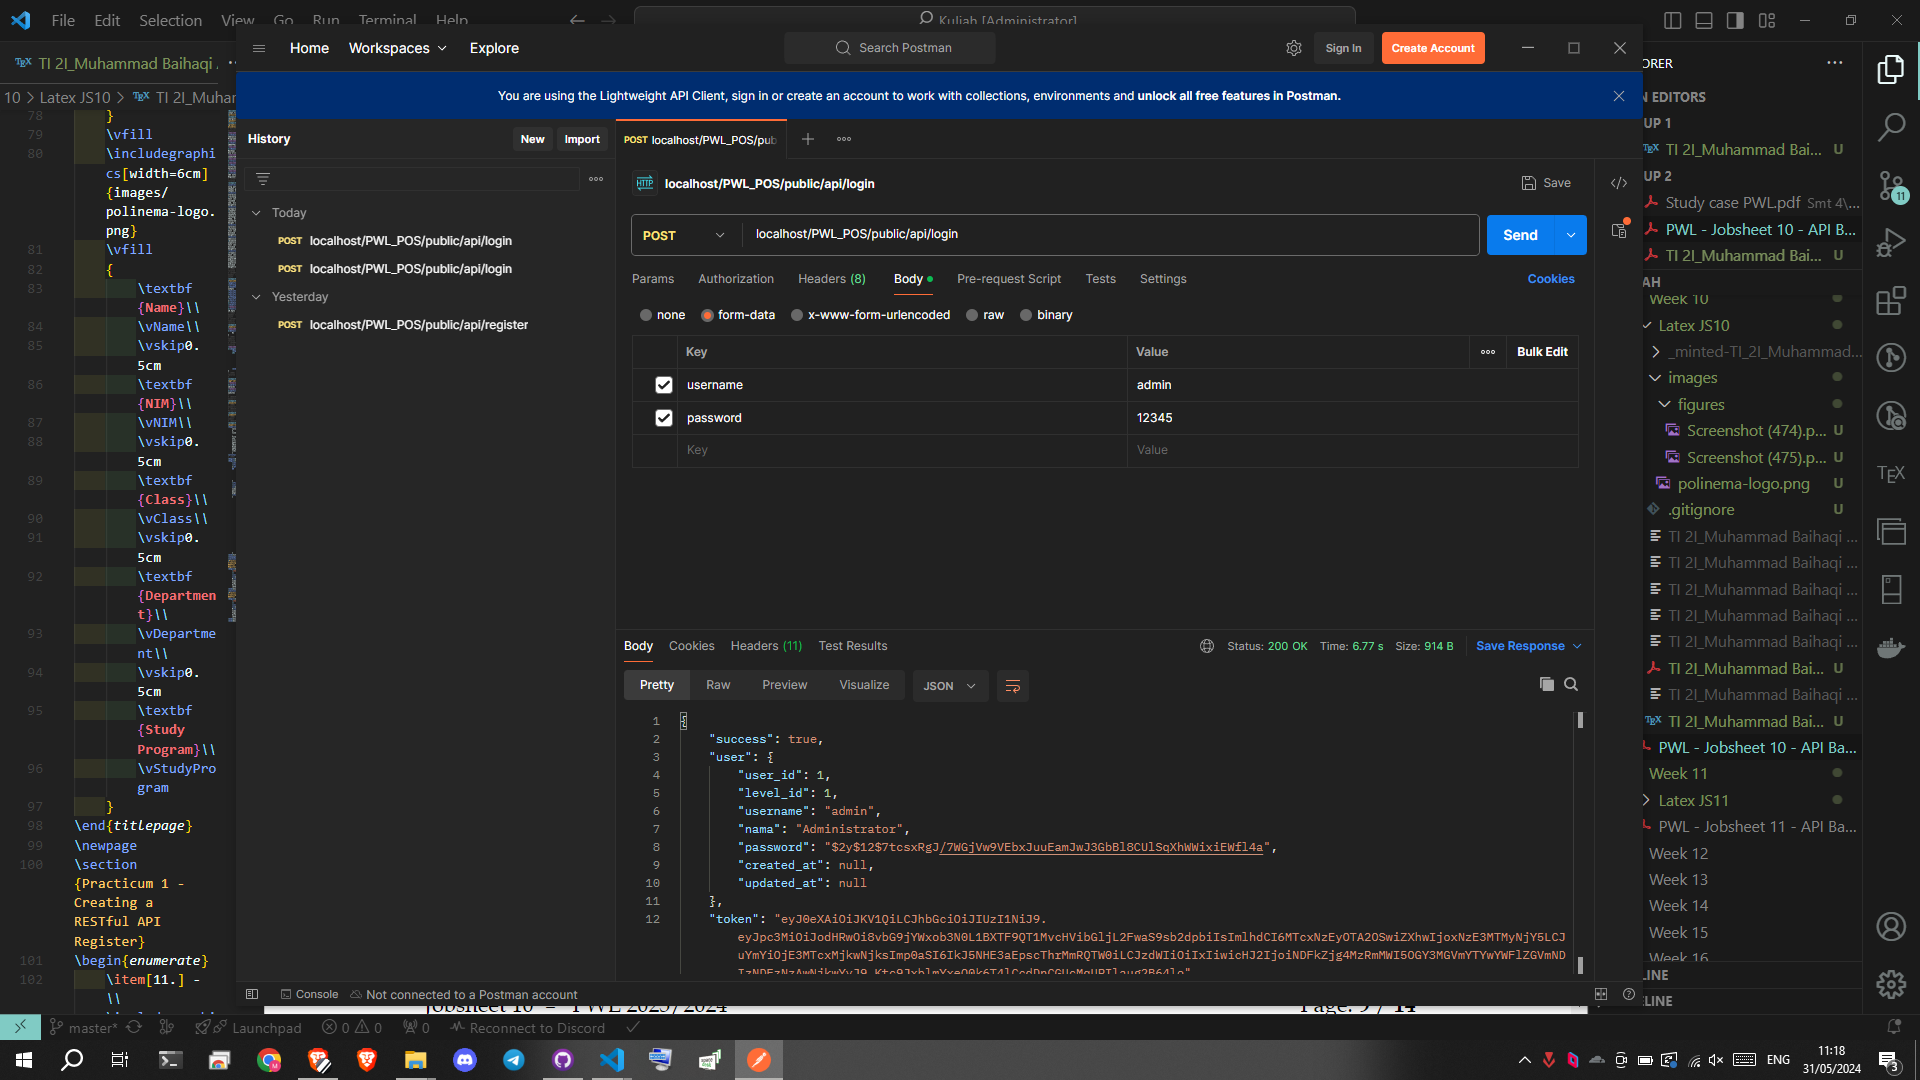
\includegraphics[width=.9\textwidth]{images/figures/Screenshot (476).png}
    \item[6.] - \\ \includegraphics[width=.9\textwidth]{images/figures/Screenshot (477).png}
    \item[7.] - \\ \includegraphics[width=.9\textwidth]{images/figures/Screenshot (478).png}
\end{enumerate}
\section{Practicum 3 - Creating a RESTful API Logout}
\begin{enumerate}
    \item[6.] - \\ \includegraphics[width=.9\textwidth]{images/figures/Screenshot (472).png}
\end{enumerate}
\section{Practicum 4 - CRUD implementation in RESTful API}
\begin{enumerate}
    \item[4.] - \\ 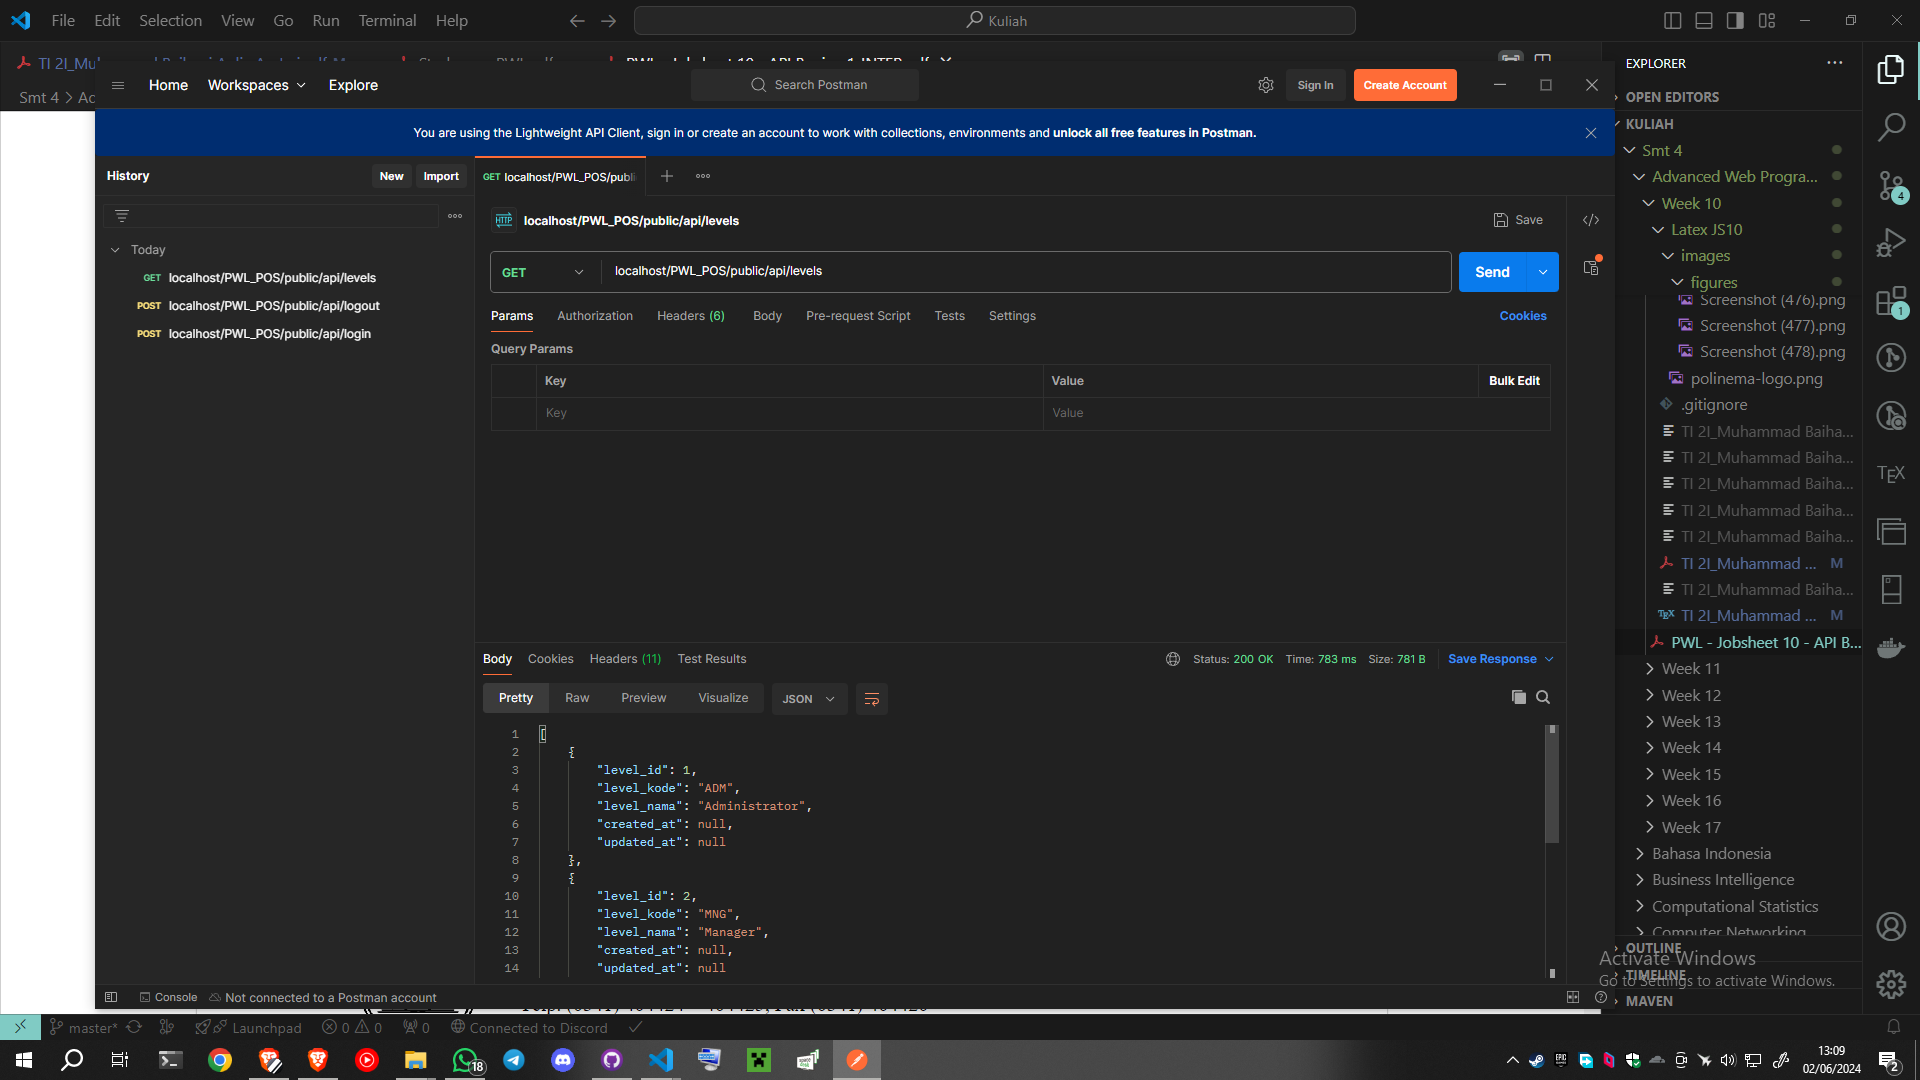
\includegraphics[width=.9\textwidth]{images/figures/Screenshot (480).png} \\ it return a json array of object of all of the record in the m\textunderscore level table
    \item[5.] - \\ \includegraphics[width=.9\textwidth]{images/figures/Screenshot (481).png} \\ it create a record for the m\textunderscore level table according to the form-data we inputed
    \item[6.] - \\ \includegraphics[width=.9\textwidth]{images/figures/Screenshot (482).png} \\ it display the detail information of the level with the coresponding id
    \item[7.] - \\ \includegraphics[width=.9\textwidth]{images/figures/Screenshot (483).png} \\ it update the value of the parameter we change accordingly
    \item[8.] - \\ \includegraphics[width=.9\textwidth]{images/figures/Screenshot (484).png} \\ it delete the data
\end{enumerate}
\url{https://github.com/G4CENeiz/PWL_POS}
\end{document}
